\chapter{Conclusion}
\label{conclusion0}

\begin{flushright}
\textit{``\,... in life we ultimately pursue, not conclusions, but beginnings.''}\\
-- Sam Tanenhaus \citep[American historian, in:][]{Tanenhaus1986}
\end{flushright}

%\newpage
%\vspace*{1ex}
\section{Summary}
\label{conclusion1}

Lore ipsum.


%\newpage
%\vspace*{1ex}
\section{Future work}
\label{conclusion2}

One can think of numerous little improvements and extras, that would help the workflow.
Among them are additional tools for topology control or mesh manipulation.
The optimization and the parallelization of the algorithms, also seem to pose legitimate research question.\\
Having said that, we want to focus the discussion on two entirely different issues.
The first question in section \ref{conclusion21} is motivated by the standards used in the industries, which are currently dealing with biggest assets and therefore would be the most likely candidates to adopt any of the presented results.
In short, the problem is, that for various reasons quad meshes are the quasi norm for many applications.
Yet it is not clear how the remeshing part could be adopted in a smart manner to provide for quad meshes.\\
The second question in section \ref{conclusion22}, reviews ideas of how the calculation of the Betti numbers could be sped up.
The main idea being, that a locally restricted algorithm would not only decrease running times but also improve the geometrical significance of our results.

\subsection{Adaption for Quad-Meshes}
\label{conclusion21}

The problem of generating high quality quad meshes from triangle meshes or point cloud data has been fairly well researched.
Including several surveys on the topic \citep[cf. ][]{Alliez2005, Hormann2007}.
The reason for the interest in quad meshes is, that it converts raw geometric data into a higher representation that is suitable for sophisticated operations like texturing, subdivision and compression.\\
Constructing good meshes is still hard task though, not only are there a series of quality criteria like 'edge-flow', 'individual element quality', etc. but their optimization often requires the consideration of global dependencies.
Therefore to implement a naïve quad meshing scheme after the stochastic vertex selection phase should be rather straight forward \citep[cf.][]{Li2009}, but doing it with good results and some flexibility in terms of what criteria to optimize isn't \citep[][]{Bommes2009}.
More importantly, whatever strategy gets deployed, it should take full advantage of the levers that are already in place.
What we mean by that is, that there are parts like loop computation that could be exploited to guide the meshing scheme.
%Bild
\begin{figure}[ht]
\centering
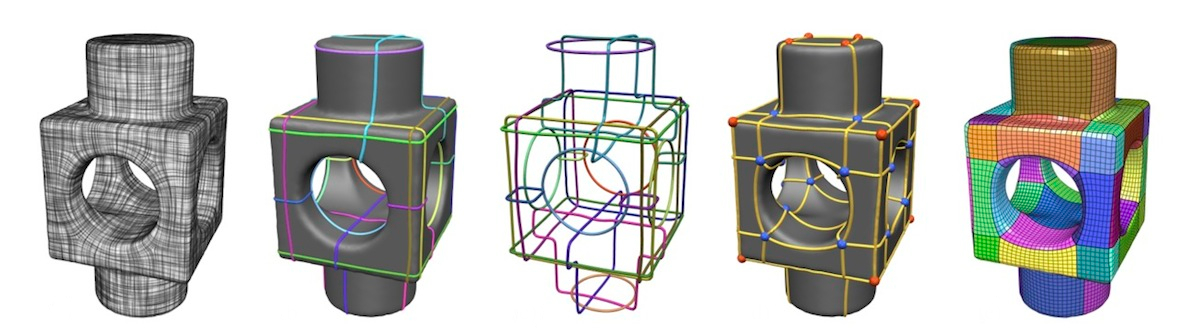
\includegraphics[width=1.0\textwidth]{dual_loop_meshing.jpg}
\caption{BLA \citep[cf.][]{Campen2012}.}
\label{fig:dual_loop_meshing}
\end{figure}\\
Just now, \textit{Campen et al.} presented a novel approach, called ``Dual Loops Meshing'', to get high quality, coarse, all-quadrilateral patch layouts on manifold surfaces \citep[][]{Campen2012}.
Their method uses a field of principal curvature directions, to get a collection of transversally crossing loops on the surface.
These loops partition the surface into polygonal regions whose valences are connected to their total curvature, see figure \ref{fig:dual_loop_meshing}.
And although we haven't analyzed the actual familiarities between their concept and the techniques we use, it is clear that they are related and could generate synergies.

\subsection{Fast $\beta^{1}$ Calculation via Decimation \& Segmentation}
\label{conclusion22}

Throughout the thesis we calculated all the Betti numbers for entire meshes, yet this seems to be unnecessary wasteful since large parts of the model are just not important, i.e. bearing $\beta^{1} = 0$.
Especially as the used pairing algorithm, described in \ref{algo:simplex_pairing}, does not scale very well.
The reason for that is, that the expansion of chain complexes in the \texttt{while loop} \,gets considerably more computational expensive as the size of the simplicial complex \mathrm{K} increases and with it, its chains.
We think that there could be ways to exclude the pricy calculation of $\beta^{2}$ in favor of smart heuristics, thereby gaining huge speed-ups.
Even if that should turn out, not to work, two further ideas could yield valuable improvements.\\
First it could be tried to quickly segment the mesh into topological meaningful parts.
Ideally one would try to dismiss as much segments, with genus null, as possible.
Thus, leaving only a smaller subset for the more involved computations.
This should be feasible since checking the topological importance is very cheap and calculated via the linear sum over the simplices.
Breaking up the problem into smaller parts provides further advantages for later stages of the process.
In case of searching for handle and tunnel loops, this would also make the tetrahedralization faster, and place the generating edges closer to the features they represent.
On top of all of that, could the smart segmentation of a mesh lead to a parallelization of the algorithm that might even lends itself to a GPU implementation -- altering the running times of these computations rather orders of magnitude than just some percentages.
%Bild
\begin{figure}[ht]
\centering
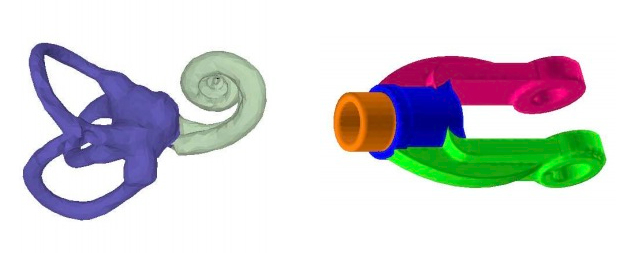
\includegraphics[width=0.60\textwidth]{betti_segmentation.jpg}
\caption{Example of topological meaningful mesh segmentations \citep[][Figure 7 \& 9]{Attene2006}.}
\label{fig:betti_segmentation}
\end{figure}\\
The second idea plays on the fact that topology does not care about the actual size of simplices but rather their connectivity.
Consequentially all invariants are retained even if the mesh has undergone drastic simplifications, as long as the simplification process preservs the topology.
On that account, accelerating the computation can be achieved by adding a step in the algorithm that strongly decimates the mesh upfront.
Equipped with a homeomorphic low polygonal representation, the actual computation of the invariants can be done much faster.
This could make it even practically relevant to drop the tetrahedralization part of the handle and tunnel loop computation all together, which in turn, could lead to better results for knotted surfaces which present a problem for the current approach.
The interesting features of the low poly model, of course, would have to be mapped to the highly detailed original mesh afterwards.
Possibly this can result in the necessity to do a further clean-up process of the mapped data, but even so this route seems to be very promising.

A preliminary search of the topic showed that, fast algorithms for the calculation of Betti numbers have been of interest for researchers since at least the early nineties \citep[cf.][]{Delfinado1993}.
However, simplification or segmentation as a preprocess hasn't been prominently featured in any of the works that we found so far.
Which is somewhat striking, for the reason that Betti numbers are often used in context of decimation.
It seems that papers in this research area are either more concerned about other aspects, like for instance 'Contour Trees', or restrict their applications to isosurfaces, alpha shapes and so on \citep[cf.][]{Pascucci2003, Konkle2003}.


